\section{User manual}
Figure~\ref{fig:router} depicts the router configuration. Three components are required to use the board as a DHCP relay:
\begin{itemize}
	\item DHCP server, assigns IP addresses to clients;
	\item DHCP client, requests an IP address;
	\item DHCP relay, bridges between the client and the server.
\end{itemize}

\begin{figure}[h]
	\centering
	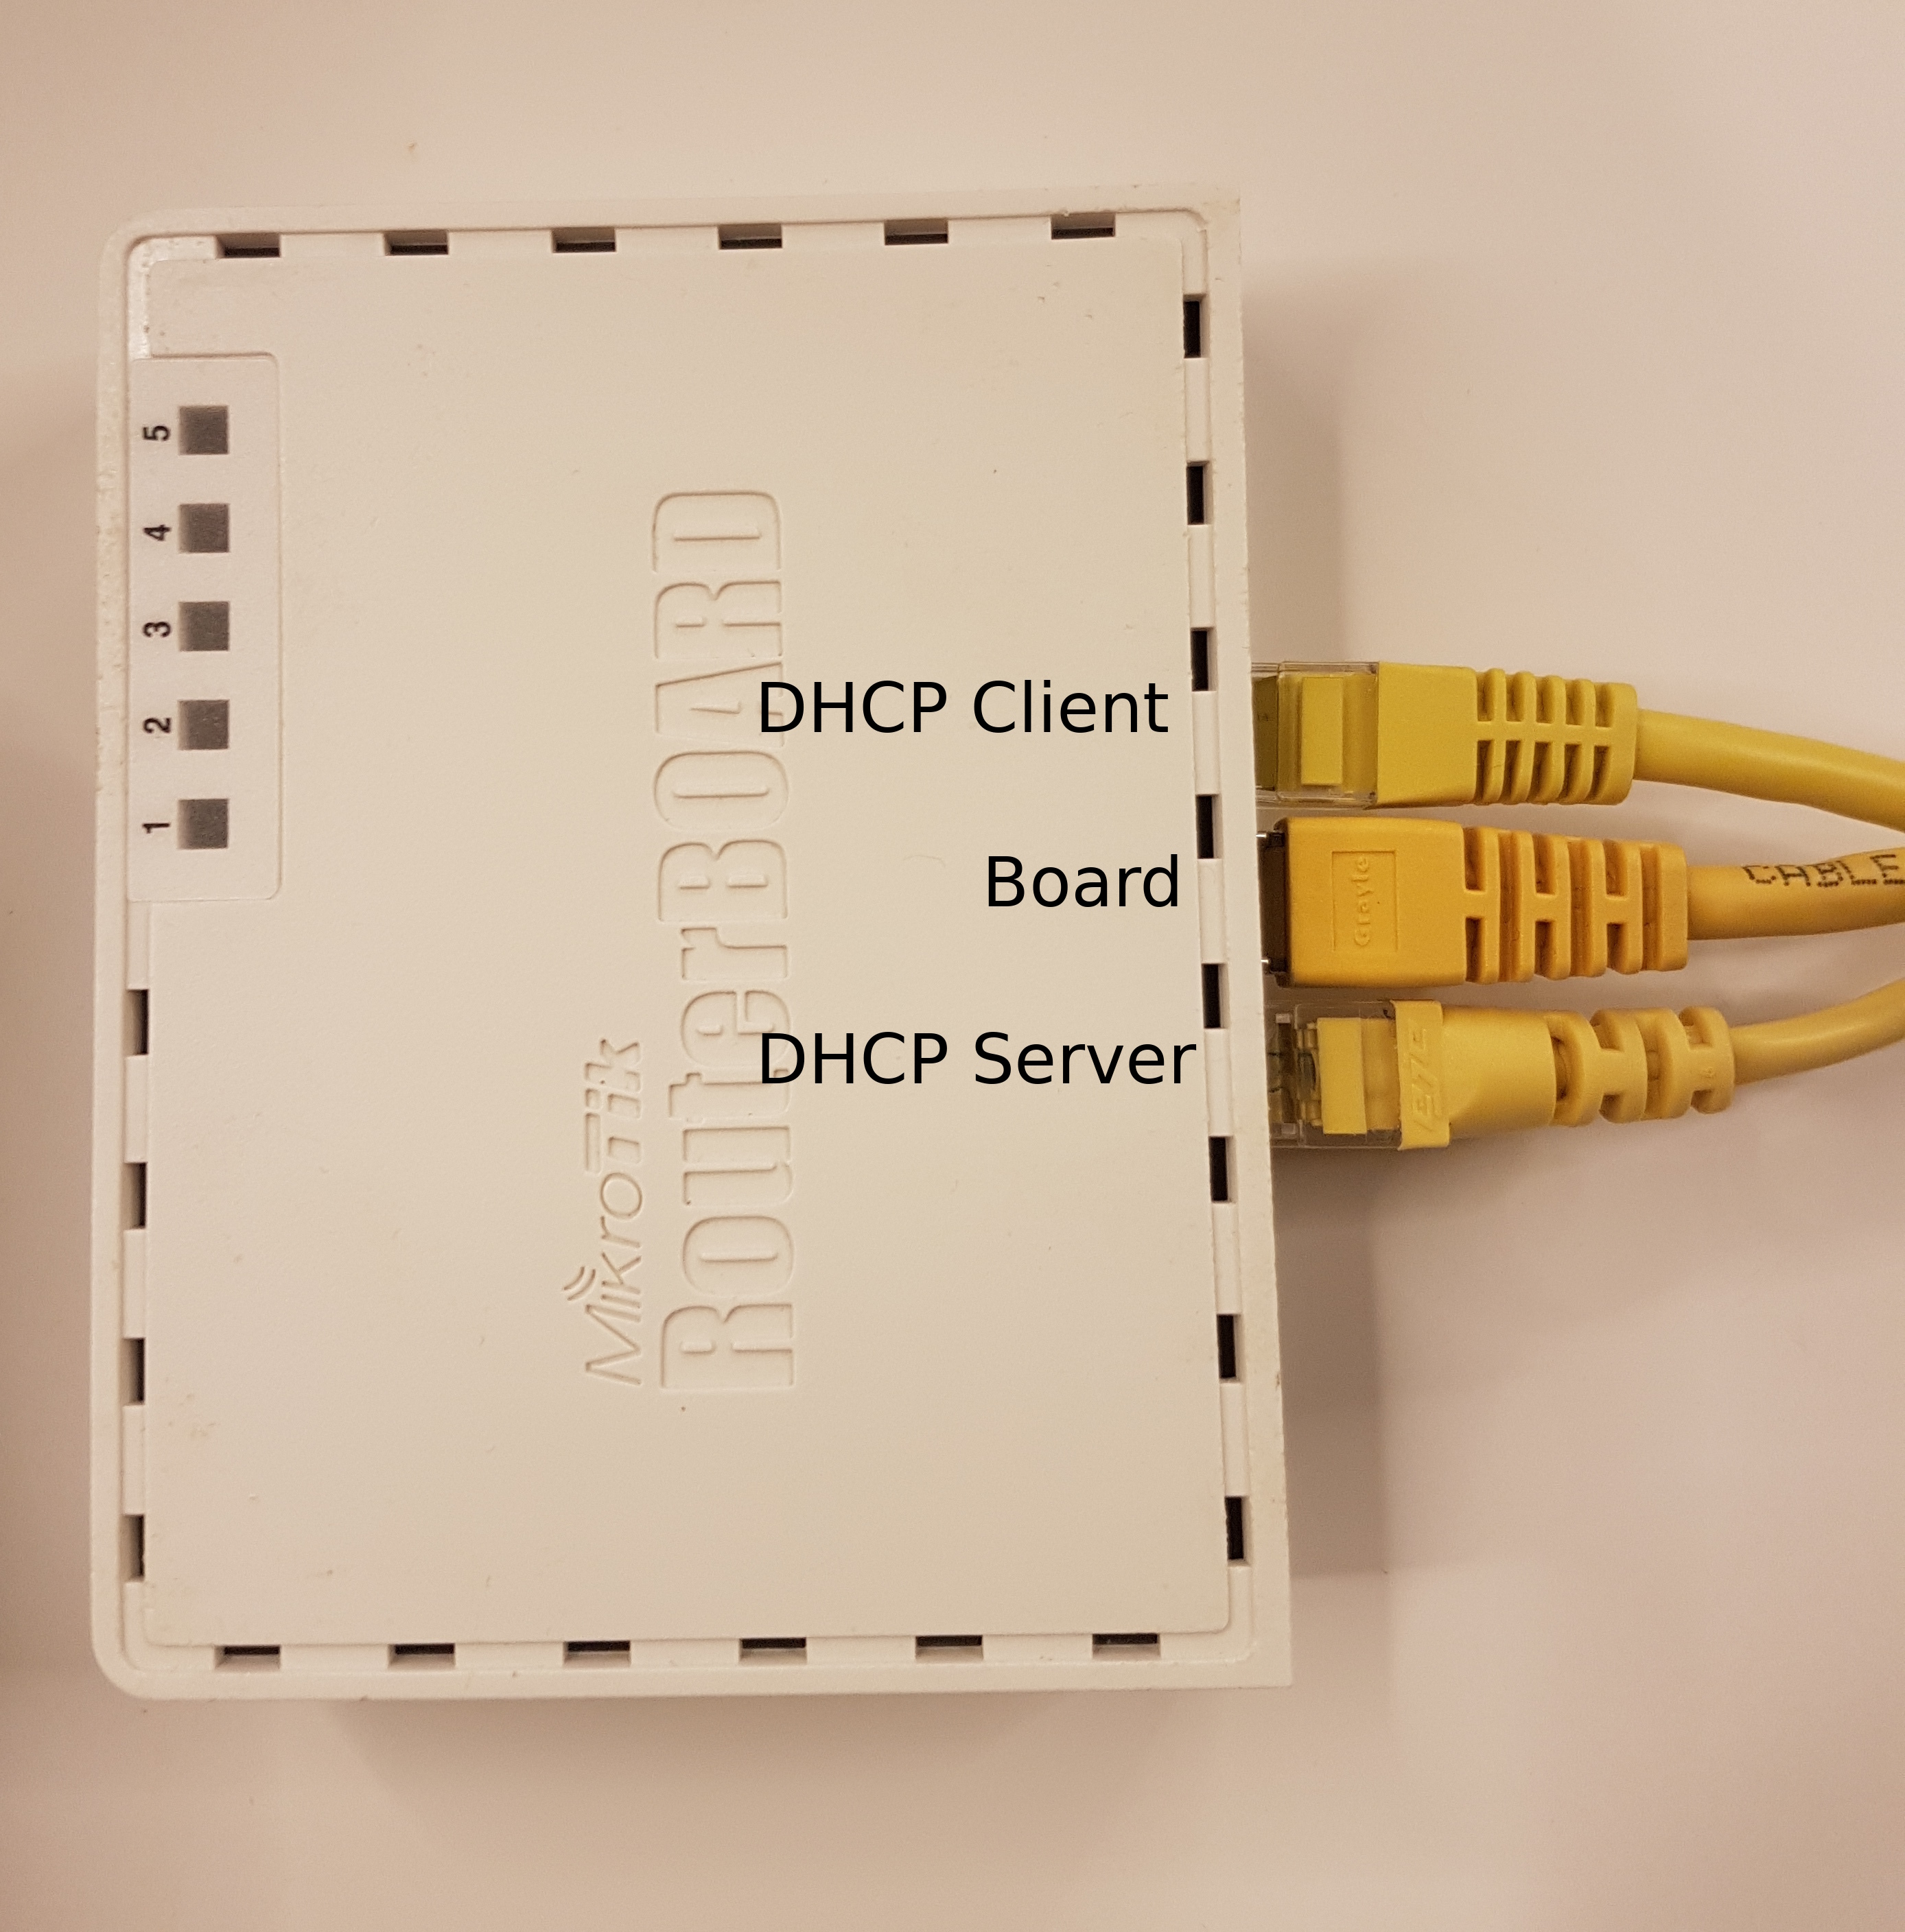
\includegraphics[scale=0.1]{images/router}
	\caption{Router configuration}
	\label{fig:router}
\end{figure}

Server and clients are supposed to belong to two different network (otherwise a relay would not be necessary, and they could communicate ``directly''). The server must be connected to Port 1. The relay and the client(s) must be connected to ports from 2 to 5. A user can use these ports interchangeably. In Figure~\ref{fig:router}, relay and client are connected to Port 2 and 3, respectively. 

You should set you Ethernet interface to require an IP address assigned dynamically (in other words, you should not specify a static IP address).